\documentclass{beamer}
\mode<presentation>
\usepackage{amsmath}
\usepackage{amssymb}
%\usepackage{advdate}
\usepackage{graphicx}
\graphicspath{{./figs/}}
\usepackage{adjustbox}
\usepackage{subcaption}
\usepackage{enumitem}
\usepackage{multicol}
\usepackage{mathtools}
\usepackage{listings}
\usepackage{url}
\def\UrlBreaks{\do\/\do-}
\usetheme{Boadilla}
\usecolortheme{lily}
\setbeamertemplate{footline}
{
  \leavevmode%
  \hbox{%
  \begin{beamercolorbox}[wd=\paperwidth,ht=2.25ex,dp=1ex,right]{author in head/foot}%
    \insertframenumber{} / \inserttotalframenumber\hspace*{2ex} 
  \end{beamercolorbox}}%
  \vskip0pt%
}
\setbeamertemplate{navigation symbols}{}

\providecommand{\nCr}[2]{\,^{#1}C_{#2}} % nCr
\providecommand{\nPr}[2]{\,^{#1}P_{#2}} % nPr
\providecommand{\mbf}{\mathbf}
\providecommand{\pr}[1]{\ensuremath{\Pr\left(#1\right)}}
\providecommand{\qfunc}[1]{\ensuremath{Q\left(#1\right)}}
\providecommand{\sbrak}[1]{\ensuremath{{}\left[#1\right]}}
\providecommand{\lsbrak}[1]{\ensuremath{{}\left[#1\right.}}
\providecommand{\rsbrak}[1]{\ensuremath{{}\left.#1\right]}}
\providecommand{\brak}[1]{\ensuremath{\left(#1\right)}}
\providecommand{\lbrak}[1]{\ensuremath{\left(#1\right.}}
\providecommand{\rbrak}[1]{\ensuremath{\left.#1\right)}}
\providecommand{\cbrak}[1]{\ensuremath{\left\{#1\right\}}}
\providecommand{\lcbrak}[1]{\ensuremath{\left\{#1\right.}}
\providecommand{\rcbrak}[1]{\ensuremath{\left.#1\right\}}}
\theoremstyle{remark}
\newtheorem{rem}{Remark}
\newcommand{\sgn}{\mathop{\mathrm{sgn}}}
\providecommand{\abs}[1]{\left\vert#1\right\vert}
\providecommand{\res}[1]{\Res\displaylimits_{#1}} 
\providecommand{\norm}[1]{\lVert#1\rVert}
\providecommand{\mtx}[1]{\mathbf{#1}}
\providecommand{\mean}[1]{E\left[ #1 \right]}
\providecommand{\fourier}{\overset{\mathcal{F}}{ \rightleftharpoons}}
%\providecommand{\hilbert}{\overset{\mathcal{H}}{ \rightleftharpoons}}
\providecommand{\system}[1]{\overset{\mathcal{#1}}{ \longleftrightarrow}}
%\providecommand{\system}{\overset{\mathcal{H}}{ \longleftrightarrow}}
	%\newcommand{\solution}[2]{\textbf{Solution:}{#1}}
%\newcommand{\solution}{\noindent \textbf{Solution: }}
\providecommand{\dec}[2]{\ensuremath{\overset{#1}{\underset{#2}{\gtrless}}}}
\newcommand{\myvec}[1]{\ensuremath{\begin{pmatrix}#1\end{pmatrix}}}
\let\vec\mathbf

\lstset{
%language=C,
frame=single, 
breaklines=true,
columns=fullflexible
}

\numberwithin{equation}{section}

\title{1.5.8}
\author{EE25BTECH11020 - Darsh Pankaj Gajare}
\begin{document}
\maketitle
% \newpage
% \bigskip
Question:\\
Find the ratio in which $\vec{P}\brak{4, 5}$ divides the line segment joining $\vec{A}\brak{2, 3}$ and $\vec{B}\brak{7, 8}$.\\
\textbf{Solution:}
\begin{table}[H]
	\centering
	\begin{center}
    \begin{tabular}{|c|c|c|} 
        \hline
            \textbf{Variable} & \textbf{Parameter} & \textbf{Value} \\ 
        \hline
            $\lVert \vec{B - A}\rVert$ & c & 5 cm \\ 
        \hline
             $\lVert \vec{C - B}\rVert$ & a & - \\ 
        \hline
             $\lVert \vec{C - A}\rVert$ & b &   -    \\
        \hline
            $\angle \vec{A}$  & -  & $45^\circ$ \\
        \hline
    \end{tabular}
\end{center}  

	\caption{Given Data}
	\label{}
\end{table}
\begin{align}
	k=\frac{\brak{\vec{A}-\vec{P}}^T\brak{\vec{P}-\vec{B}}}{\norm{\vec{P}-\vec{B}}^2}
\end{align}
Substituting values,
\begin{align}
	k=\frac{\myvec{-2 & -2}\myvec{-3\\-3}}{\norm{\myvec{-3\\-3}}^2}  =\frac{2}{3}
\end{align}
\begin{figure}[H]
\centering
	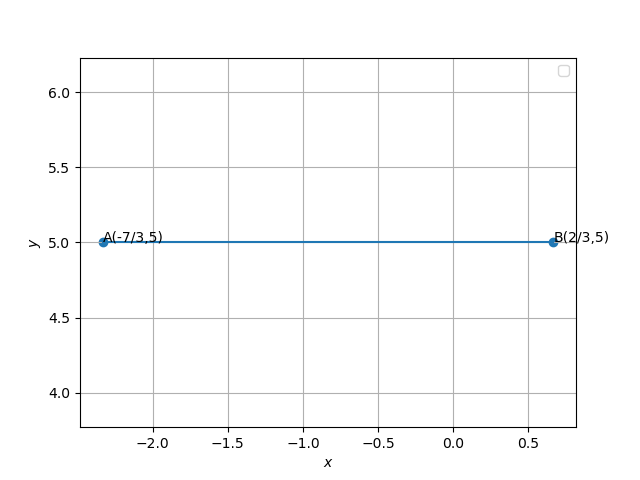
\includegraphics[scale=0.5]{img}
	\caption*{}
	\label{img}
\end{figure}
\end{document}
